\chapter{Otras protecciones eléctricas de AT}
\section{Protección direccional de sobreintensidad de neutro 67N}
\begin{itemize}
	\item Se emplea en redes de distribución con baja intensidad de defecto:
	redes con neutro aislado o de alta impedancia
	\item Son relés direccionales: miden la intensidad y tensión homopolares
	\begin{itemize}
		\item Tensión homopolar: por TT conectado en triángulo abierto
		\item Intensidad homopolar: por TI toroidal o suma
	\end{itemize}
	\item Se conectan en todas las salidas de la subestación
	\item Selectividad por distinto ángulo de la intensidad de defecto en la
	salida en falta respecto a las salidas intactas
\end{itemize}

\begin{figure}[H]
	\centering
	\begin{minipage}[b]{0.45\linewidth} % Ancho de la primera figura
		\centering
		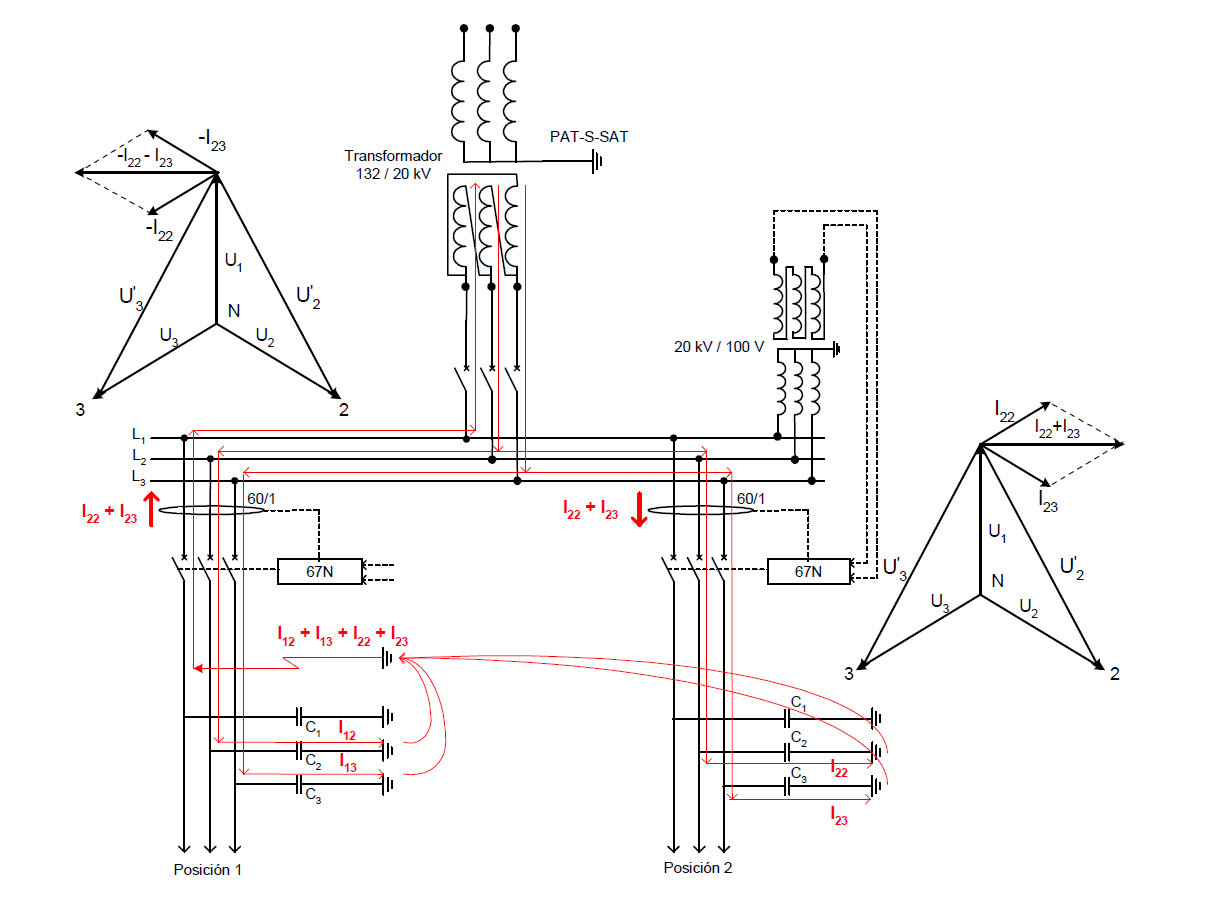
\includegraphics[width=\linewidth]{Images/67}
		\caption{Figura 67}
		\label{fig:67}
	\end{minipage}
	\hspace{0.05\linewidth} % Espacio entre las figuras
	\begin{minipage}[b]{0.45\linewidth} % Ancho de la segunda figura
		\centering
		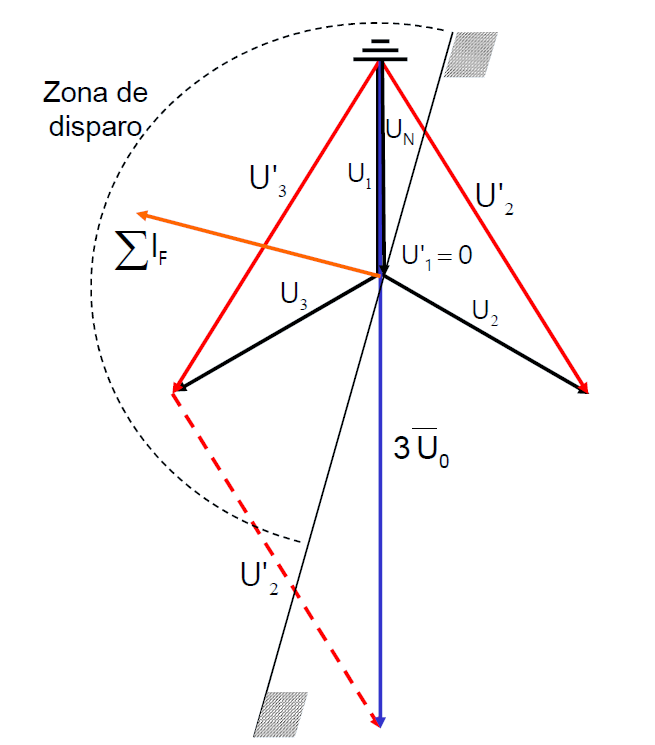
\includegraphics[width=\linewidth]{Images/68}
		\caption{Figura 68}
		\label{fig:68}
	\end{minipage}
\end{figure}
\begin{equation}
	\sum I_f=-I_22-I_23
\end{equation}

Ajuste de la protección: $< U_0 - I_d > = \ang{110}$ inductivo
\section{Protección diferencial}
Es una protección que solo debería disparar si la falta es interna en el equipo. Si la falta es externa no debería disparar, pero por errores de módulo y fase puede ocurrir.
\begin{figure}[H]
	\centering
	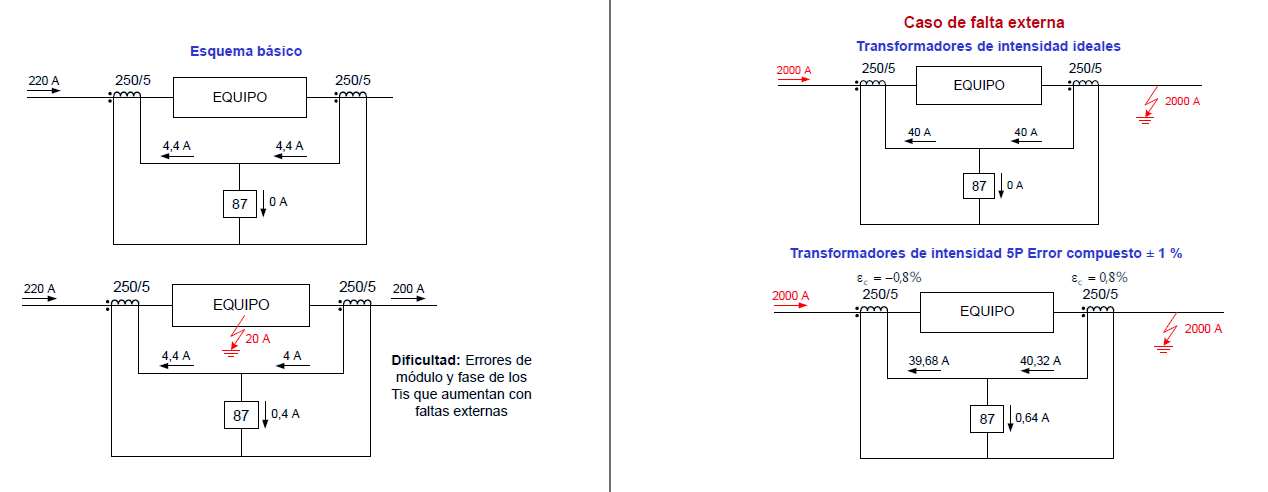
\includegraphics[width=1\linewidth]{Images/69}
	\label{fig:69}
\end{figure}

Para solucionar esto se hace que la sensibilidad del relé disminuya con el incremento de la corriente de frenado. Se usan Relés diferenciales de pendiente porcentual.
\begin{itemize}
	\item Para zonas cercanas a la intensidad
	nominal los TI no se saturan
	\item Para intensidades superiores a la
	nominal la sensibilidad disminuye al
	aumentar la intensidad de frenado
\end{itemize}

El grupo de conexión (índice horario) del transformador
introduce un desfase entre las corrientes
primaria y secundaria.
\begin{figure}[H]
	\centering
	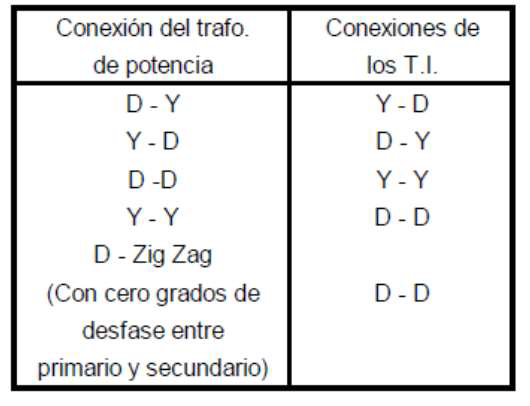
\includegraphics[width=0.4\linewidth]{Images/70}
	\label{fig:70}
\end{figure}

Dificultades adicionales:
\begin{itemize}
	\item Es necesario (para grupos de conexión Dy ó Yd) filtrar las corrientes
	homopolares para evitar la actuación del relé ante faltas a tierra externas
	\begin{itemize}
		\item Mediante conexiones en triángulo de los TIs
		\item Con filtros de intensidad homopolar
	\end{itemize}
	\item En la conexión del transformación se produce una corriente transitoria que no
	debe disparar el relé
	\item En la sensibilidad del relé se debe tener en cuenta:
	\begin{itemize}
		\item El error debido a la diferencia de corrientes del transformador de potencia
		\item Los errores de los TIs (especialmente en condiciones transitorias)
		\item La diferencia de errores en los TIs
		\item El efecto producido por la regulación en carga
	\end{itemize}
\end{itemize}
\subsection{Ejemplo para conexión Ydn}
\begin{figure}[H]
	\centering
	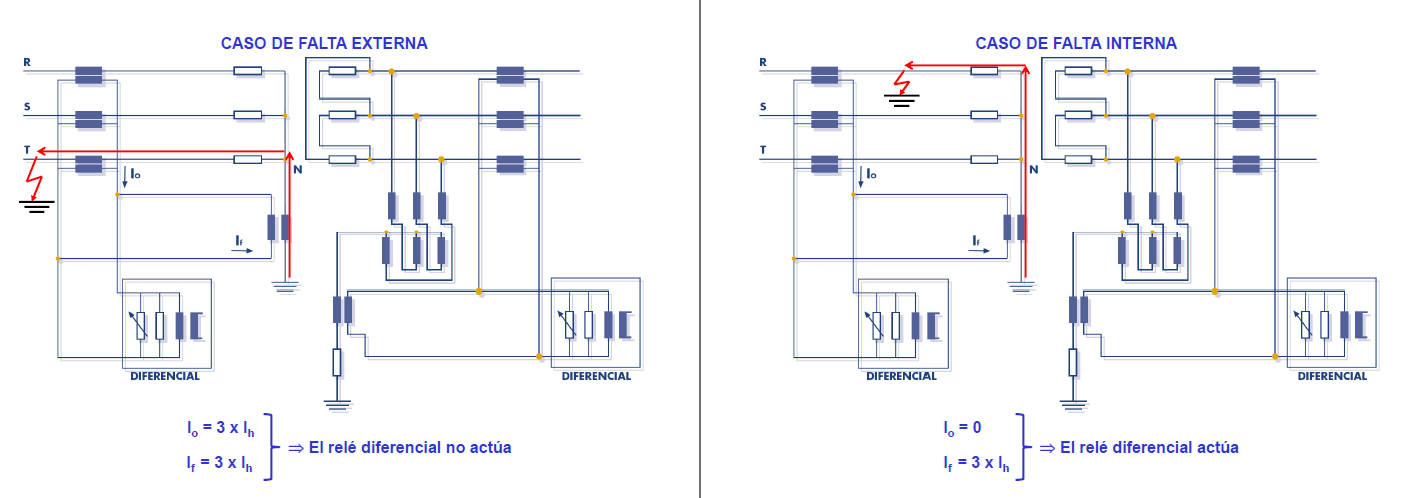
\includegraphics[width=1\linewidth]{Images/71}
	\label{fig:71}
\end{figure}

\section{Protección de distancia 21}
En condiciones de falta la impedancia de la línea es proporcional a la distancia a la falta y suele ser de carácter inductivo. Para ello, se usa el relé de distancia 21:
\begin{itemize}
	\item Mide la impedancia de la línea y da orden de disparo si la impedancia es menor a un valor
	ajustado, denominado “alcance”
	\item El TT puede conectarse del “lado de línea” o del “lado de barras”. La conexión del lado de línea
	se utiliza cuando es necesario sincronizar las tensiones de línea y barras para cerrar el interruptor
	\item Si el alcance es del 100 \% puede abrir para una falta fuera de la línea produciéndose sobrealcance y perdiendo selectividad.
\end{itemize}
\subsection{Alcance para disparo sin retardo: 80 – 90 \% de la longitud total de la línea}
Evita sobre alcance debido a imprecisiones de la medida de impedancia y el estado de carga de la línea.
\begin{figure}[H]
	\centering
	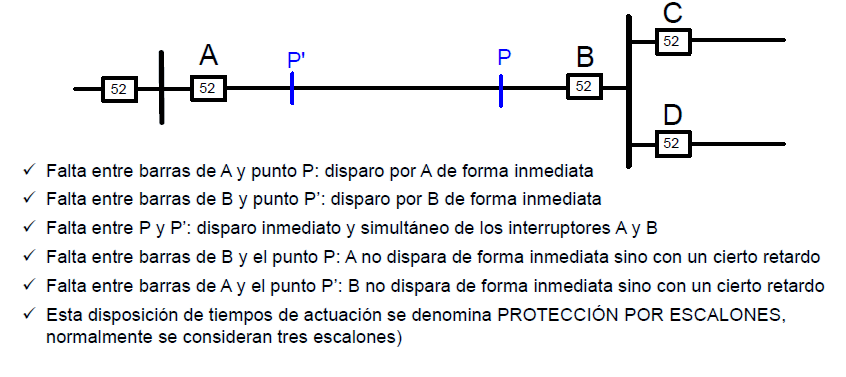
\includegraphics[width=0.7\linewidth]{Images/73}
	\label{fig:73}
\end{figure}

\subsection{Protección por escalones}
\begin{itemize}
	\item Primer escalón: disparo sin retardo de faltas en el 80 – 90 \% de la longitud de la línea (evita sobrealcance)
	\item Segundo escalón: disparo para faltas en el 20 – 10 \% de la longitud de la línea no protegida por el primer
	escalón y del 25 – 30 \% de la siguiente línea (evita subalcance) y respaldo remoto para la protección de barras
	\item Tercer escalón: actúa como respaldo remoto del interruptor siguiente en la cadena de protección: A respalda a
	C, etc. y como respaldo local de los interruptores situados en el otro lado de su embarrado: A respalda a Z, etc.
	\item Habitualmente los dos primeros escalones son direccionales y el tercer escalón no
\end{itemize}
\section{Esquemas de protecciones de subestación de distribución}
\begin{figure}[H]
	\centering
	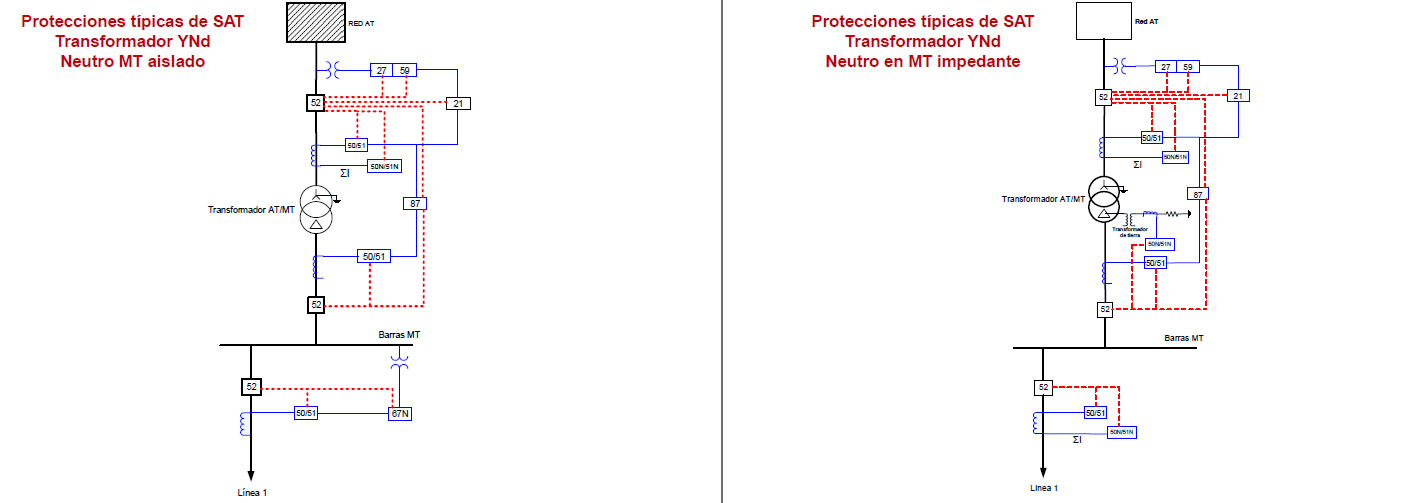
\includegraphics[width=1\linewidth]{Images/72}
	\label{fig:72}
\end{figure}
